%=========== main.tex (converted for phdnotes class) ===========
\documentclass[a4paper,12pt]{PhDNotes} % Using custom class

% Load phdnotes style (contains chapter design, TOC styling, etc.)
\usepackage{Notation}

% Bibliography with IEEE style
\usepackage[backend=biber,style=ieee]{biblatex}
\addbibresource{ReferenceTest/ReferencesTest.bib} % Your BibTeX file

% Metadata
\title{PhD Research Notes}
\author{Farhan Aizuddin}
\date{\today}

\begin{document}

% Roman numbered frontmatter
\frontmatter
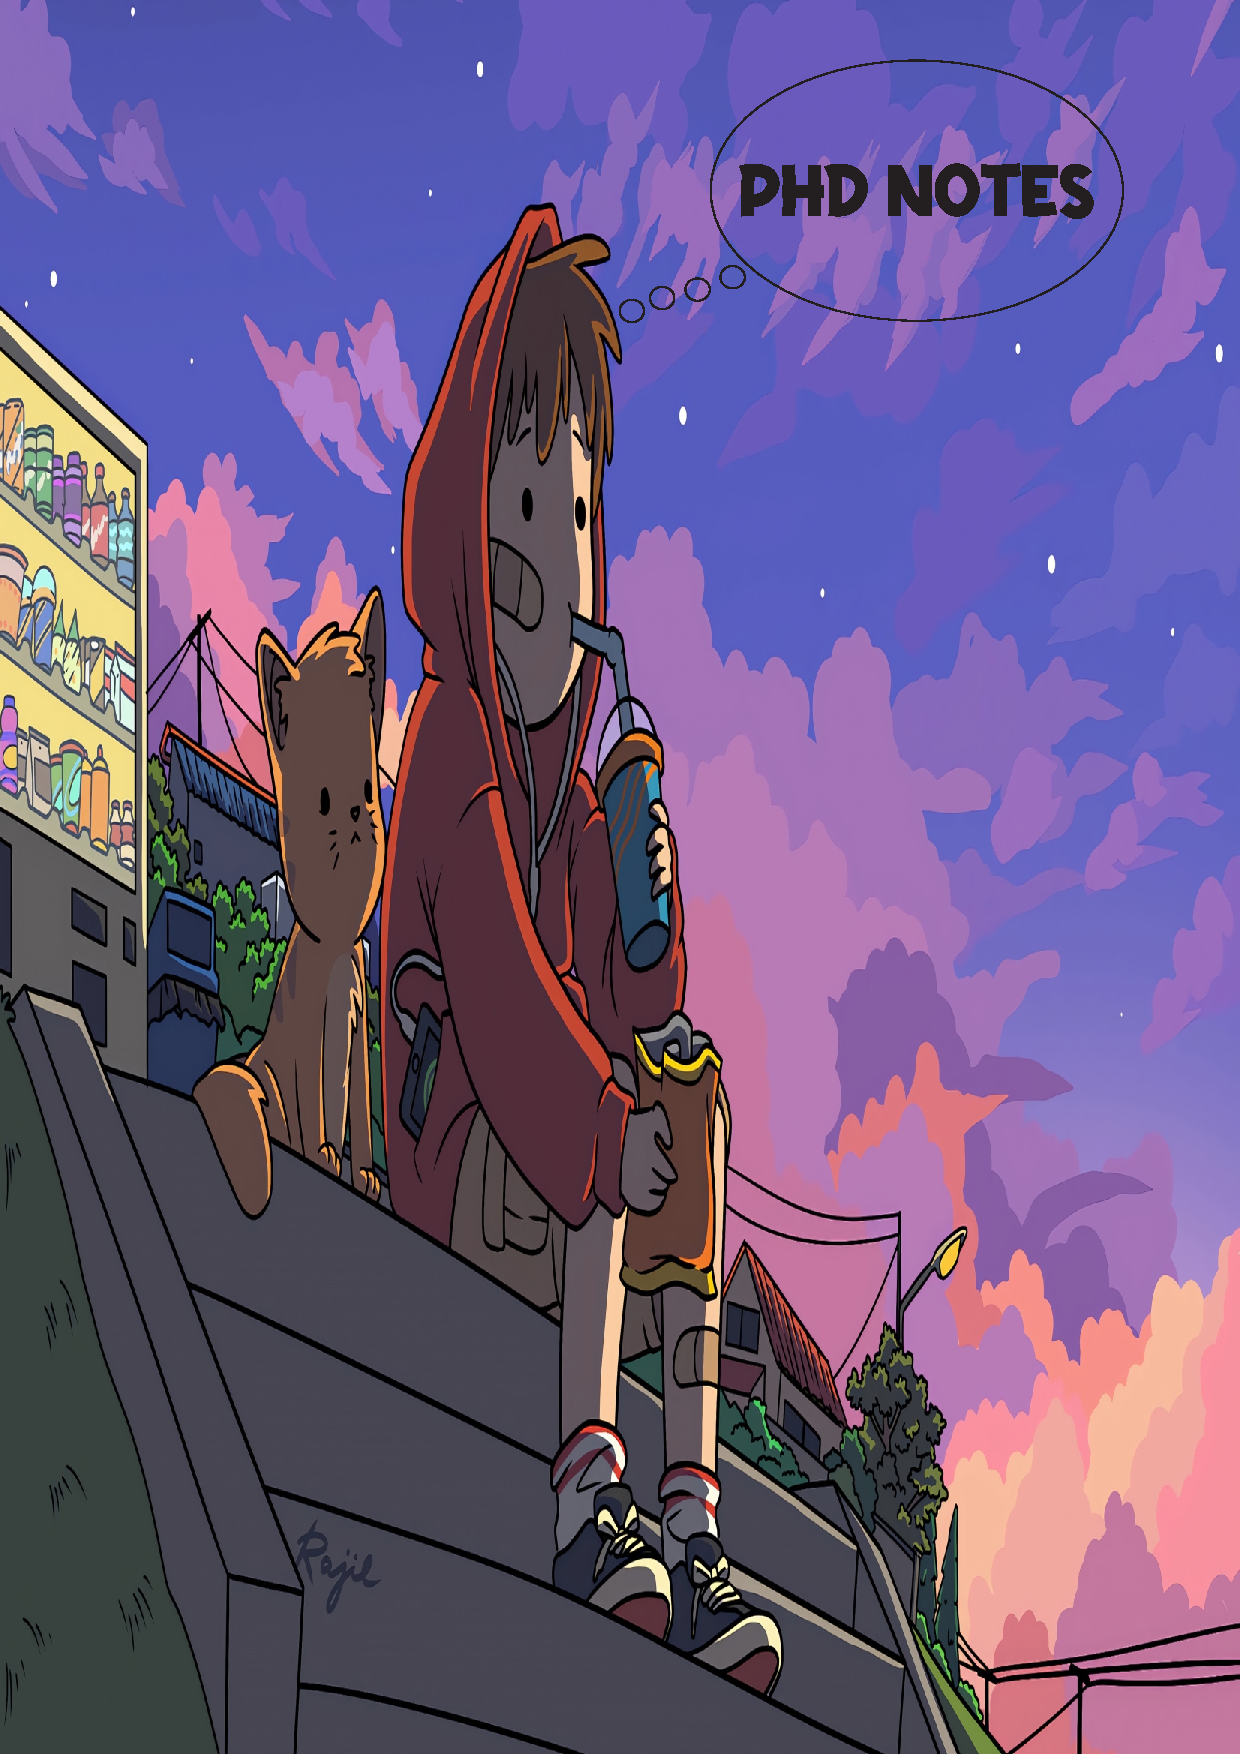
\includepdf[pages={1}]{PhD_Notes_Cover}
\tableofcontents*

% Arabic numbered content
\mainmatter

% Include paper chapters
\chapter{Paper-Based Digital Microfluidics}
\section{Summary}
This paper elucidates a novel methodology for the fabrication of digital microfluidic (DMF) devices predicated on the utilisation of paper as a substrate, thereby addressing the inherent limitations of conventional DMF systems, notably their cost and the complexities associated with clean-room-based fabrication processes.\\

The authors posit that the proposed paper-based DMF paradigm offers a facile, rapid, and cost-effective alternative, enabling the creation of disposable devices suitable for individual experiments, thus mitigating issues such as adsorption and dielectric breakdown.

\section{Key Points of the Paper}

\subsection{Novel Fabrication Method} 
The paper introduces a new approach to fabricating digital microfluidic (DMF) devices using paper as the primary substrate, along with graphite for electrodes, adhesive tape as a dielectric layer, and commercially available water repellants as hydrophobic coatings. This method aims to overcome the limitations of traditional DMF fabrication, which often involves expensive materials and complex, time-consuming clean-room processes.

\subsection{Low-Cost and Accessible Materials} 
A key feature of this work is the exclusive use of low-cost, readily available materials. Paper serves as an inexpensive and flexible substrate. Graphite spray provides a simple means of creating conductive electrodes. Adhesive tape functions as the dielectric layer. Two different commercial water repellants (Nevosil Si-7100 and Avam rain repellant) are explored as cost-effective alternatives to materials like Teflon-AF.

\subsection{Simplified Fabrication Process}
The proposed fabrication procedure is significantly simpler, faster, and lower in cost compared to conventional methods. It involves template creation using a laser cutter, direct patterning of graphite electrodes by spraying over the template, application of adhesive tape as the dielectric, and finally, treatment with a hydrophobic substance. This out-of-clean-room approach enhances the accessibility of DMF technology.

\subsection{Functional Device Demonstration} 
The authors successfully demonstrate the basic functionalities of the fabricated paper-based DMF device, including droplet movement and merging, with droplet volumes ranging from 15 to 50 \textmugreek L. The merging of \(\ce{NaOH}\) and phenolphthalein droplets, resulting in a colour change, visually confirms the on-chip reaction capability.

\subsection{Low-Cost High-Voltage Actuation} 
To actuate the droplets via electrowetting on dielectric (EWOD), a custom-designed, low-cost, and portable high-voltage supply circuit is presented. This circuit, costing less than \$10 and powered by a 6V battery, utilises a switching flyback transformer from a CRT display and a 555 timer IC to generate the necessary voltage (approximately 700 $V_{AC}$) for droplet manipulation.

\subsection{Advantages of Paper as a Substrate} The use of paper offers several advantages, including its low cost, availability in various forms, flexibility, biocompatibility, and disposability. Furthermore, paper's compatibility with lamination and common printing methods opens avenues for simple, fast, and potentially massive patterning of conductive electrodes. The potential for merging paper-based DMF with conventional paper-based microfluidics to create hybrid devices is also highlighted.

\subsection{Addressing Limitations of PCB-based DMF}
The paper explicitly addresses drawbacks associated with using printed circuit boards (PCBs) as substrates in DMF devices, such as the presence of deep trenches between electrodes that can impede droplet movement. The proposed paper-based DMF avoids this issue as the graphite electrodes can penetrate the paper, resulting in a more planar surface.

\subsection{Performance Comparison of Hydrophobic Layers} 
Two different hydrophobic materials, Nevosil Si-7100 and Avam rain repellant, were evaluated. Nevosil Si-7100 exhibited better performance in terms of treatment, while Avam rain repellant, although more cost-effective and readily available, proved harder to treat uniformly on the adhesive tape.

\subsection{Limitations and Future Research Directions} 
The authors acknowledge certain limitations of the current paper-based DMF system, including temperature constraints (unsuitable for experiments above 200 °C), the physical limitations of paper, restrictions on high-grade dielectric materials, and limitations in electrode resolution and droplet volume. Future research is suggested to focus on reducing electrode size and inter-electrode gaps through finer patterning techniques (such as printing), decreasing the required actuation voltage by using thinner dielectric layers, and developing closed paper-based DMF configurations.

\section{Conclusion}
In conclusion, this paper presents a significant step towards democratising DMF technology by introducing a highly accessible and cost-effective fabrication method using commonplace materials. \\

The successful demonstration of fundamental droplet manipulation on the proposed paper-based platform underscores its potential for various applications, particularly in resource-limited settings, while also highlighting areas for future development and refinement.\\

Figure \ref{Abadian_2014} summarizes the contents of this paper.
\begin{figure}[h!]
    \centering
    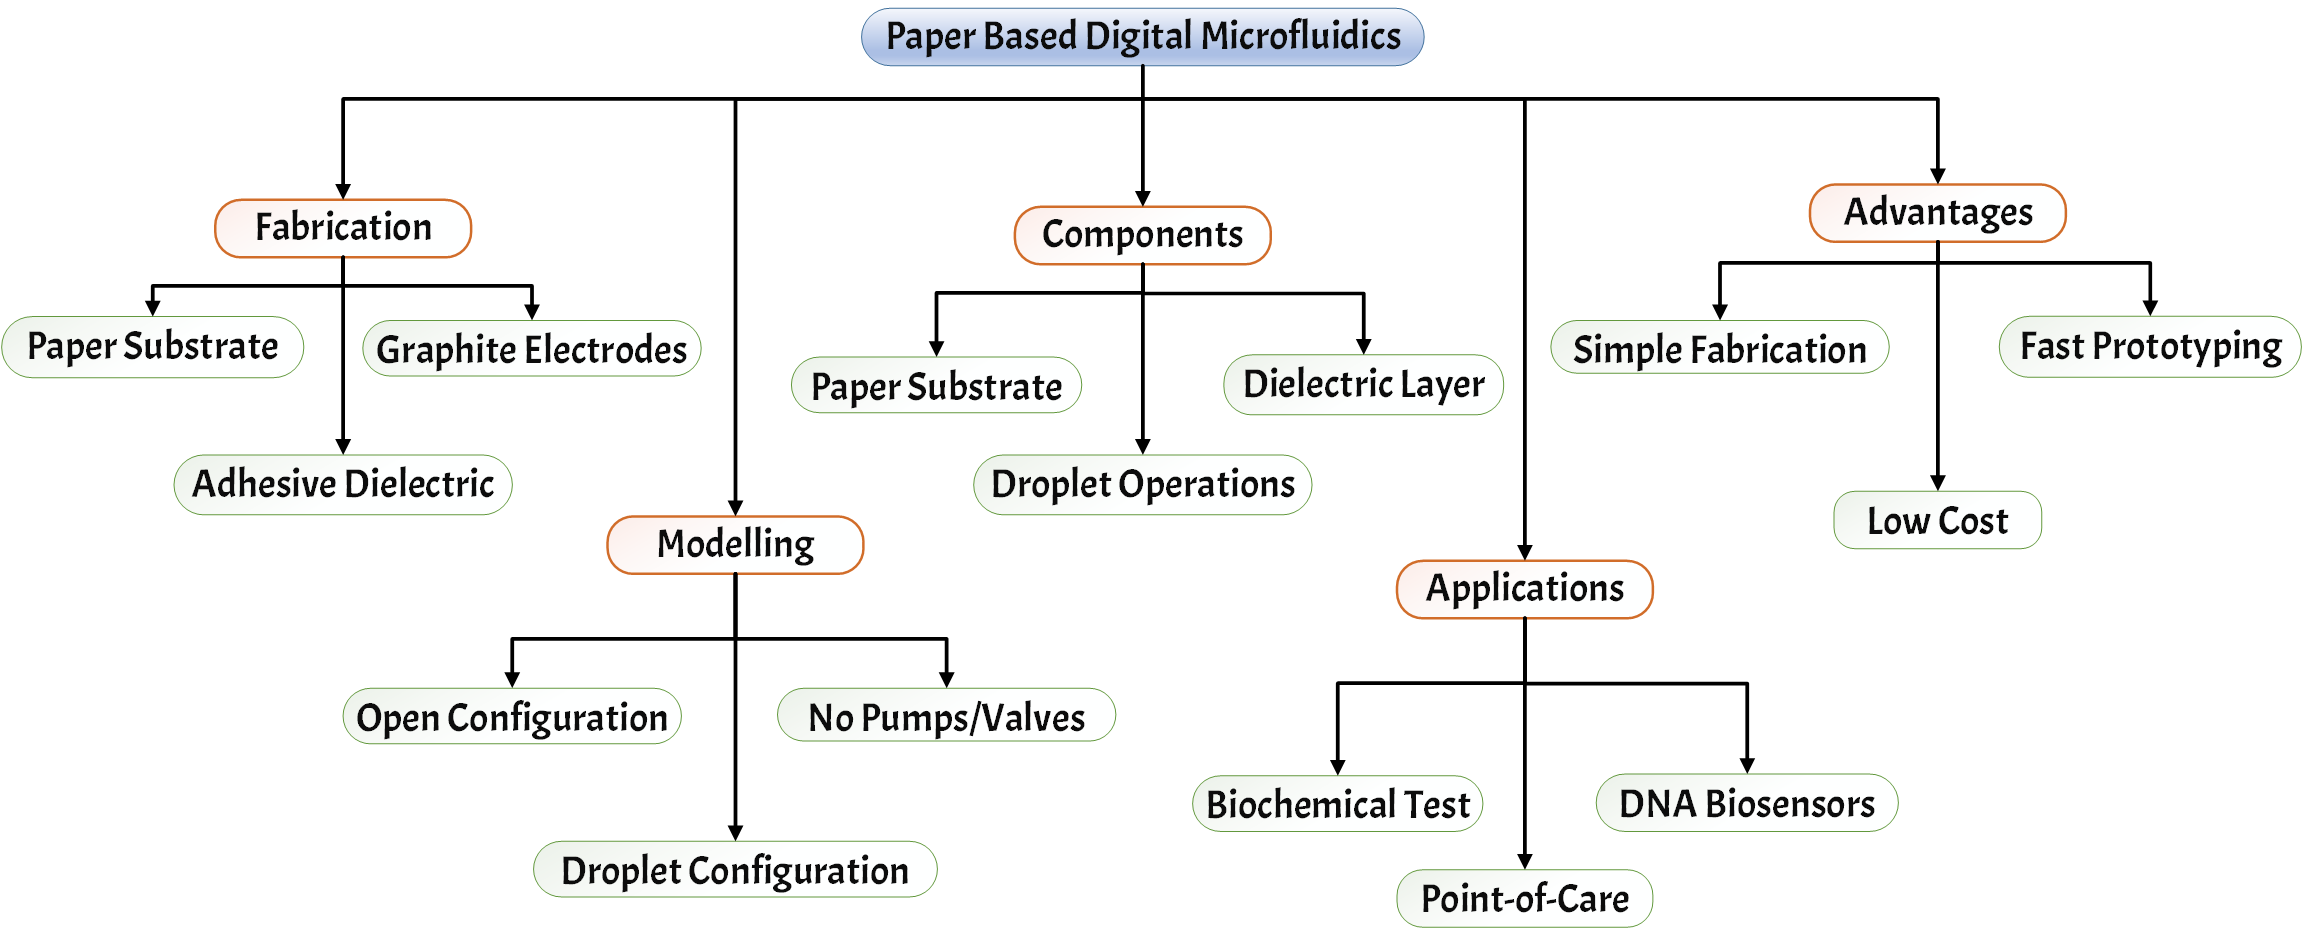
\includegraphics[width=\textwidth]{Abadian_Jafaradi_2014.png}
    \caption{Structure of Paper-based Digital Microfluidics technology.}
    \label{Abadian_2014}
\end{figure}

\chapter[Hybrid paper‑based microfluidics]{Hybrid paper‑based microfluidics: combination of paper‑based analytical device (\textmugreek PAD) and digital microfluidics (DMF) on a single substrate}

\section{Summary}
This paper presents a significant contribution to the field of microfluidics by introducing and experimentally validating a novel hybrid paper-based microfluidic (HPMF) device. This innovative platform strategically integrates the functionalities of paper-based analytical devices (\textmugreek PADs) and digital microfluidics (DMF) onto a single substrate, aiming to overcome the inherent limitations associated with each individual technology.\\

The authors posit that this synergistic combination enhances the capabilities of microfluidics in point-of-care (POCT) diagnostics by enabling controlled droplet manipulation for preprocessing on the DMF component, followed by versatile sensing and post-processing on the µPAD component.

\section{Keypoints}
\subsection{Focus}
The paper introduces a novel hybrid paper-based microfluidic (HPMF) device that integrates a digital microfluidic (DMF) platform with a microfluidic paper-based analytical device (µPAD) on a single paper substrate. This combination aims to leverage the strengths of both technologies while mitigating their respective limitations. \newpage
\subsection{\textmugreek PAD vs DMF}
Table \ref{PlatformComparison} describes the pros and cons of \textmugreek PAD and DMF.
\begin{table}[h!]
    \centering
    \caption{Comparison between \textmugreek PAD and DMF}
    \label{PlatformComparison}
    \begin{tblr}{
        width = \linewidth,
        colspec = {Q[75]Q[23]Q[406]Q[23]Q[408]},
        cell{1}{3} = {c},
        cell{1}{5} = {c},
        hline{1,5} = {-}{0.08em},
      }
      Platform &  & \textmugreek PAD &  & DMF\\
      Pros &  & {\labelitemi\hspace{\dimexpr\labelsep+0.5\tabcolsep}Low-cost~\\\labelitemi\hspace{\dimexpr\labelsep+0.5\tabcolsep}Simple to fabricate} &  & \labelitemi\hspace{\dimexpr\labelsep+0.5\tabcolsep}Precise manipulation of droplets through electrowetting on dielectric (EWOD)\\
       &  &  &  & \\
      Cons &  & {\labelitemi\hspace{\dimexpr\labelsep+0.5\tabcolsep}Lack of precise control over fluid flow\\\hspace*{0.5\leftmargin}\labelitemii\hspace{\dimexpr\labelsep+0.5\tabcolsep}hindering their application in multistep processes requiring sample preparation} &  & {\labelitemi\hspace{\dimexpr\labelsep+0.5\tabcolsep}
       Typically uses non-paper substrates\\\labelitemi\hspace{\dimexpr\labelsep+0.5\tabcolsep}Faces challenges in post-processing steps\\\hspace*{0.5\leftmargin}\labelitemii\hspace{\dimexpr\labelsep+0.5\tabcolsep}Particularly sensing \\\hspace*{1\leftmargin}\labelitemiii\hspace{\dimexpr\labelsep+0.5\tabcolsep}Separation of fluids from electrodes by a dielectric layer}
      \end{tblr}
    \end{table}
%\chapter[Optimization of Device Geometry in Single-Plate DMF\\{\normalfont Abdelgawad et al. (2009)}]%
{Optimization of Device Geometry in Single-Plate Digital Microfluidics\\[1ex]{\normalfont Abdelgawad et al. (2009)}}

\section{Paper Overview}
\includefig[h!]{0.8}{Abdelgawad_2019_Overview }{Paper overview}
\includefig[h!]{0.8}{Abdelgawad_2019_GeometryComparison}{6 grounding geometries comparison}
%\include{AnotherFolder/AnotherPaper}  % Add more as needed

% Bibliography
\backmatter
\printbibliography

\end{document}
